%\documentclass[a4paper]{jarticle} 
\documentclass[dvipdfmx,a4paper]{jsarticle}
\usepackage{tikz}
\usepackage{amsmath}
\usepackage{amssymb}
\topmargin = 0mm
\oddsidemargin = 5mm
\textwidth = 152mm
\textheight = 240mm


% サブセクションを 問1,問2 にする設定
\renewcommand{\thesection}{[\arabic{section}]}

% サブサブセクションを (1),(2)にする設定
\renewcommand{\thesubsection}{(\arabic{subsection})}
% (i),(ii)なら \arabic を \roman に変える。    (a),(b)なら \alph

\renewcommand{\thesubsubsection}{(\roman{subsubsection})}



% 大問2の3番目の計算式のラベルを (2.3) にする設定
% 計算式の参照には \eqref{eq:hoge} を使う
\makeatletter
  \renewcommand{\theequation}{\arabic{subsection}.\arabic{equation}}
  \@addtoreset{equation}{subsection}
\makeatother

% --------------------------------------------------------------------
\begin{document}

% タイトル
\begin{center}
\textbf{\huge{数学2D演習 第2回}}
\end{center}

%名前
\begin{flushright}
工学部電気電子工学科3年 03200489 末吉七海\\
\end{flushright}

% --------------------------------------------------------------------
% 問1
\section{}

%(1)
\subsection{}

辺々2乗して、$(|a| + |b|) ^2 \geq | a+b| ^2  \geq(|a| - |b|) ^2$を示せば良い。\\
$a = |a|\exp{(i\theta_a)}, b = |b|\exp{(i\theta_b)}$とおくと、
\begin{align*}
|a + b|^2 &= \bigl||a|\exp{(i\theta_a)} + |b|\exp{(i\theta_b)}\bigr|^2\\
&= \bigl||a|(\cos{\theta_a} + i\sin{\theta_a}) + |b|(\cos{\theta_b} + i\sin{\theta_b})\bigr|^2\\
&= \bigl|\bigl(|a|\cos{\theta_a} + |b|\cos{\theta_b}\bigr) + i(\bigl(|a|\sin{\theta_a} + |b|\sin{\theta_b}\bigr)\bigr|^2\\
 &= \bigl(|a|\cos{\theta_a} + |b|\cos{\theta_b}\bigr)^2 + \bigl(|a|\sin{\theta_a} + |b|\sin{\theta_b}\bigr)^2\\
 &= |a|^2\cos^2{\theta_a} + 2|a||b|\cos{\theta_a}\cos{\theta_b} + |b|^2\cos^2{\theta_b} + |a|^2\sin^2{\theta_a} + 2|a||b|\sin{\theta_a}\sin{\theta_b} + |b|^2\sin^2{\theta_b}\\
 &= |a|^2 + |b|^2 + 2|a||b|\cos{(\theta_a -\theta_b)}
\end{align*}

$-1\leq\cos{(\theta_a -\theta_b)}\leq 1$より、
\begin{align*}
|a|^2 + |b|^2 + 2|a||b| &\geq |a|^2 + |b|^2 + 2|a||b|\cos{(\theta_a -\theta_b)} \geq |a|^2 + |b|^2 - 2|a||b|\\
\therefore \quad (|a| + |b|)^2 &\geq |a + b|^2 \geq (|a| - |b|)^2
\end{align*}

ただし、m、nを整数として、\\
\qquad 左の等号が成立するのは、$cos{(\theta_a -\theta_b)}=1$すなわち$\theta_a = \theta_b+2m\pi$の時\\
\qquad 右の等号が成立するのは、$cos{(\theta_a -\theta_b)}=-1$すなわち$\theta_a = \theta_b+(2n-1)\pi$の時\\
以上より、与不等式は示された。\\


%(2)
\subsection{}
\begin{align*}
1^2 - \Bigl|\frac{a-b}{1-\bar a b}\Bigr|^2 &= 1 - \frac{a-b}{1-\bar a b}\overline{\frac{a - b}{1 - \bar a b}}\\
&= 1 - \frac{a-b}{1 - \bar a b}\frac{\bar a - \bar b}{1 - a \bar b}\\
&= \frac{(1 - \bar a b)(1 - a \bar b) - (a-b)(\bar a - \bar b)}{(1 - \bar a b)(1 - a \bar b)}\\
&= \frac{1 - a \bar b - \bar a b + a \bar a b \bar b - a \bar a + a \bar b + \bar a b - b \bar b}{(1 - \bar a b)(1 - a \bar b)}\\
&= \frac{1 + a \bar a b \bar b - a \bar a - b \bar b}{(1 - \bar a b)(1 - a \bar b)}\\
&= \frac{1 - |a|^2 - |b|^2 + |a|^2|b|^2}{|1 - \bar a b|^2}\\
&= \frac{(1 - |a|^2)(1 - |b|^2)}{|1 - \bar a b|^2}\\
&\geq 0 \qquad(\because |a|^2<1, |b|^2<1, |1 - \bar a b| \geq 0)\\
\therefore \quad \Bigl|\frac{a-b}{1-\bar a b}\Bigr|^2 &> 1^2\\
\therefore \quad \Bigl|\frac{a-b}{1-\bar a b}\Bigr| &> 1\qquad(\because|\frac{a-b}{1-\bar a b}\Bigr|>0)
\end{align*}
以上より与不等式は示された。\\


%(3)
\subsection{}
(1)の三角不等式を繰り返し用いると、
\begin{align*}
|\lambda_1a_1 +\lambda_2a_2 + \cdots +\lambda_na_n| &< |\lambda_1a_1| + |\lambda_2a_2| + \cdots + |\lambda_na_n|\\
&= \lambda_1|a_1| + \lambda_2|a_2| + \cdots + \lambda_n|a_n|\\
&< \lambda_1 + \lambda_2 + \cdots + \lambda_n\\
&= 1
\end{align*}

以上より与不等式は示された。\\

%(4)
\subsection{}
複素平面乗における、$|z-a| + |z+a| = 2|c|$の幾何学的意味について考えると、\\
$z$は$a$と$-a$を焦点とし、焦点からの距離の輪が$2|c|$の楕円上に分布している。\\
よって、$|a| \leq|c|\Rightarrow$$|z-a| + |z+a| = 2|c|$を満たす$z\in \mathbb{C}$が存在すると言える。\\

次に、逆を示す。\\
\begin{align*}
2|c| &= |z-a| + |z+a| = |z-a| + |-z-a|\\
&\geq |z-a+(-z-a)| \qquad (\because 三角不等式)\\
&= 2|a|\\
\therefore |c| &\geq |a|
\end{align*}
以上より示された。\\

ここで、$|a| \leq|c|$の時、$|z-a| + |z+a| = 2|c|$を図示すると下の図のようになる。\\

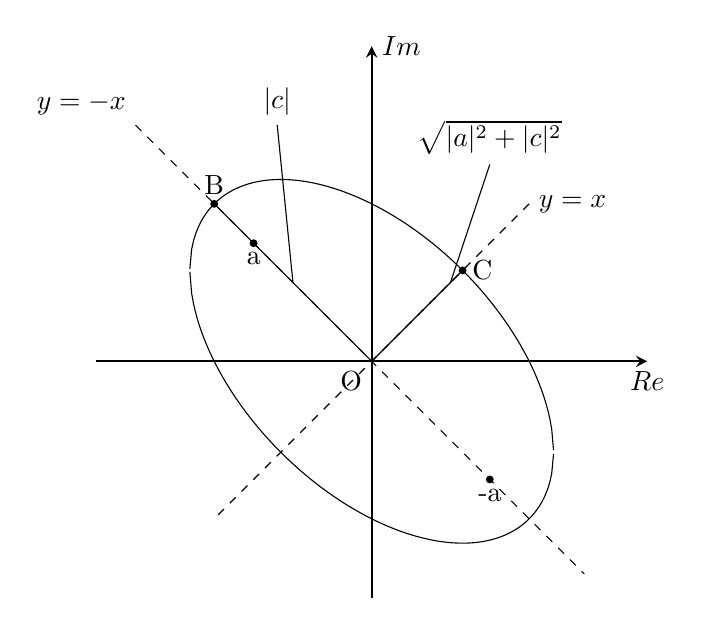
\begin{tikzpicture}
 \coordinate[label=below left:O] (O) at (0,0); %原点O
 \coordinate (XS) at (-3.5,0); %x軸最小
 \coordinate (XL) at (3.5,0); %x軸最大
 \coordinate (YS) at (0,-3); %y軸最小
 \coordinate (YL) at (0,4); %y軸最大
 \draw[thick,->,>=stealth] (XS)--(XL) node[below] {$Re$}; %x軸
 \draw[thick,->,>=stealth] (YS)--(YL) node[right] {$Im$}; %y軸
 
 \draw [samples = 200, domain=-4/sqrt(3):4/sqrt(3)] plot(\x, {- \x / 2  +  sqrt(16 -  3 * (\x) ^2 ) / 2});
 \draw [samples = 200, domain=-4/sqrt(3):4/sqrt(3)] plot(\x, {- \x / 2 - sqrt(16 -  3 * (\x) ^2 ) / 2});
 \draw[dashed] (-3,3)node[above left]{$y = -x$}--(2.7,-2.7);
 \draw[dashed] (2,2)node[right]{$ y = x$}--(-2,-2);
 \draw (-2, 2)--(0,0);
 \draw (-1,1)--(-1.2,3)node[above]{$|c|$};
 \draw (0,0)--({2/sqrt(3)},{2/sqrt(3)});
 \draw (-1.5, 1.5) node[below]{a};
 \draw (1.5, -1.5) node[below]{-a};
 \draw (-2,2) node[above]{B};
 \draw ({2/sqrt(3)},{2/sqrt(3)}) node[right]{C};
 \draw(1,1)--(1.5,2.5)node[above]{$\sqrt{|a|^2 + |c|^2}$};
 \fill (-1.5, 1.5) circle(0.05);
 \fill (1.5, -1.5) circle(0.05);
 \fill(-2,2) circle(0.05);
 \fill({2/sqrt(3)},{2/sqrt(3)}) circle(0.05);
\end{tikzpicture}

$|z|$は点Bで最大値、点Cで最小値をとり、 \\
\quad $|z|$の最大値は楕円の長軸長で$|c|$\\
\quad $|z|$の最小値は楕円の短軸長で$\sqrt{|c|^2 - |a|^2}$\\

%[2]
\section{}
%(1)
\subsection{}
\subsubsection{$e^z$}
$z = x + iy$、$e^z = u + iv$とおくと、

\begin{align*}
e^z &= e^{x+iy} \\
&= e^xe^{iy}\\
&= e^x(\cos{y} + i\sin{y})
\end{align*}
より、
\begin{align*}
u = e^x\cos{y}, \qquad v = e^x\sin{y}\\
\begin{cases}
\partial_x u = e^x\cos{y}, \qquad \partial_y v = e^x\cos{y}\\
\partial_y u = -e^x\sin{y}, \qquad -\partial_x v = -e^x\sin{y}
\end{cases}
\end{align*}

以上よりCR方程式は成立していることがわかるので、$e^z$は微分可能である。\\

\subsubsection{$\ln z$}
$z = re^{i\theta}$、$\ln z = u + iv$とおくと、
\begin{align*}
\ln{z} &= ln{(re^{i\theta})} \\
&= \ln{r} + i(\theta + 2\pi n)\qquad ( n\in\mathbb{Z})
\end{align*}
より、
\begin{align*}
u = \ln{r}, \qquad v = \theta + 2\pi n
\end{align*}

$r\neq 0$において、
\begin{align*}
\begin{cases}
\partial_r u = \frac{1}{r}, \qquad \frac{1}{r}\partial_\theta v = \frac{1}{r}\\
\frac{1}{r}\partial_\theta u = 0, \qquad -\partial_r v = 0
\end{cases}
\end{align*}

以上より、$r\neq 0$においてCR方程式は成立していることがわかるので、$\ln z$は原点以外の全ての点において微分可能である。\\

\subsubsection{$e^{\bar z}$}
$z = x + iy$、$e^{\bar z} = u + iv$とおくと、

\begin{align*}
e^{\bar z} &= e^{x-iy} \\
&= e^xe^{-iy}\\
&= e^x(\cos{y} - i\sin{y})
\end{align*}
より、
\begin{align*}
u = e^x\cos{y}, \qquad v = -e^x\sin{y}\\
\begin{cases}
\partial_x u = e^x\cos{y}, \qquad \partial_y v = -e^x\cos{y}\\
\partial_y u = -e^x\sin{y}, \qquad -\partial_x v = e^x\sin{y}
\end{cases}
\end{align*}

以上よりCR方程式は成立しないことがわかるので、$e^{\bar z}$は微分不可能。\\

%(2)
\subsection{}
\subsubsection{}
$f(z) = u(x,y) + iv(x,y)\quad(z =x +iy)$は微分可能であることから、CR方程式が成立するので、
\begin{eqnarray}
\label{1}
\partial_x u &= \partial_y v\\
\label{2}
\partial_x v &= -\partial_y u
\end{eqnarray}

(\ref{1})の両辺をx、yで微分するとそれぞれ、
\begin{eqnarray}
\label{3}
\partial_{xx} u &= \partial_{yx} v\\
\label{4}
\partial_{xy} u &= \partial_{yy} v
\end{eqnarray}

同様に、(\ref{1})の両辺をx、yで微分すると、
\begin{eqnarray}
\label{5}
\partial_{xx} v &= -\partial_{yx} u\\
\label{6}
\partial_{yx} v &= -\partial_{yy} u
\end{eqnarray}

$\partial_{yx} v = \partial_{xy} v$が成り立つので、(\ref{3})、(\ref{6})より、
\begin{eqnarray}
\partial_{xx} u = -\partial_{yy} u \nonumber\\
\label{7}
\therefore (\partial_{xx}+\partial_{yy}) u = 0
\end{eqnarray}

$\partial_{yx} u = \partial_{xy} u$が成り立つので、(\ref{4})、(\ref{5})より、
\begin{eqnarray}
\partial_{xx} v = -\partial_{yy} v \nonumber\\
\label{8}
\therefore (\partial_{xx}+\partial_{yy}) v = 0
\end{eqnarray}

(\ref{7}), (\ref{8})より、u, vはいずれも調和関数であると言える。\\

\subsubsection{}
f(z)の導関数は微分する向きによらないので、
\begin{align*}
f'(z) = \partial_x f(z) &= \partial_x u(x, y) + i\partial_x v(x, y)\\
&= 0\\
f'(z) = \partial_y f(z) &= \partial_y u(x, y) + i\partial_y v(x, y)\\
&= 0
\end{align*}

実部と虚部をそれぞれ比較して、
\begin{align*}
\partial_x u(x, y) = \partial_y u(x, y) &= \partial_x v(x, y) = \partial_y v(x, y) = 0\\
\therefore \quad u(x, y) &= const. \qquad v(x, y) = const.\\
\therefore \quad f(z) &= const.
\end{align*}

以上より題意は示された。\\

\subsubsection{}
$f(z) = u(x, y) + i v(x, y)$とおくと、$|f(z)| = const.$ より $u^2 + v^2 = const.$
両辺x, yで微分すると、それぞれ
\begin{eqnarray}
\label{9}
\partial_x(u^2 + v^2) = 2\bigl(u(\partial_x u) + v(\partial_x v)\bigr) = 0\\
\label{10}
\partial_y(u^2 + v^2) = 2\bigl(u(\partial_y u) + v(\partial_y v)\bigr) = 0
\end{eqnarray}

CR方程式より、
\begin{eqnarray}
\label{11}
\partial_x u &= \partial_y v\\
\label{12}
\partial_y u &= -\partial_x v
\end{eqnarray}

(\ref{10}), (\ref{11}), (\ref{12})より、
\begin{equation}
\label{13}
u(-\partial_x v) + v(\partial_x u) = 0
\end{equation}

(\ref{9}), (\ref{13})より、$u=v =0$を除いて、
\begin{equation}
\label{14}
\partial_x u = \partial_x v = 0
\end{equation}

(\ref{14})、CR方程式より、
\begin{equation}
\label{15}
\partial_y u = \partial_y v = 0
\end{equation}

(\ref{14}), (\ref{15})が導かれ、これは(\ref{14})で除いた$u=v =0$においても成り立つので、\\
前問と同様に$f(z) = const.$\\
以上より題意は示された。\\


%[3]
\section{}
D内の任意の点$\alpha$に対して$|f(\omega)| > |f(\alpha)|$となる$\omega \in D$が存在することを示す。\\
$\alpha$を中心として、f(z)をTaylor展開すると、
$$
f(z) = f(\alpha) + f'(\alpha)(z-\alpha) + f''(\alpha)(z-\alpha)^2 + \cdots
$$
ただし、f(z)は定数ではないので、$f'(\alpha) \neq 0$\\
$\omega = \alpha + \delta e^{i\theta}(\delta > 0,  \theta in \mathbb{R})$を考えると、
三角不等式より、
\begin{align*}
|f(\omega)| &\geq |f(\alpha) + f'(\alpha) (\omega -\alpha)| - |f''(\alpha)(\omega - \alpha)^2 + \cdots |\\
&= |f(\alpha) + f'(\alpha) (\delta e^{i\theta})| - |f''(\alpha)(\delta e^{2i\theta}) + f'''(\alpha)(\delta e^{3i\theta}) + \cdots |\\
&= |f(\alpha)| + \delta f'(\alpha) - \delta ^2 |f''(\alpha) + f'''(\alpha)(\omega - \alpha) + \cdots |
\end{align*}

十分小さい$\delta$を考えるとき、第3項以降は無視して良いので、
$$
|f(\omega)| - |f(\alpha)| \geq \delta |f'(\alpha)| > 0
$$

以上より題意は示された。\\


%[4]
\section{}

%(1)
\subsection{}
A→Bは$t = 1+it (-1 \leq 1)$、B→Cは$t = -t+i (-1 \leq 1)$、C→Dは$t = -1-it (-1 \leq 1)$、\\D→Aは$t = t -i (-1 \leq 1)$と変数変換できる。

\subsubsection{$f(z) = z$}
\begin{align*}
\int_\Gamma\mathrm d z f(z) &= \int_{AB}\mathrm d z f(z) +  \int_{BC}\mathrm d z f(z) +  \int_{CD}\mathrm d z f(z) + \int_{DA}\mathrm d z f(z)\\
&= \int_{AB}\mathrm d z z +  \int_{BC}\mathrm d z z +  \int_{CD}\mathrm d z z + \int_{DA}\mathrm d z z\\
&= \int_{-1}^{1} (i\mathrm d t)(1 + it) + \int_{-1}^{1} (-\mathrm d t)(-t + i) + \int_{-1}^{1} (-i\mathrm d t)(-1 - it) + \int_{-1}^{1} (\mathrm d t)(t - i) \\
&= 2i - 2i + 2i - 2i\\
&= 0
\end{align*}

\subsubsection{$f(z) = z^2$}
\begin{align*}
\int_\Gamma\mathrm d z f(z) &= \int_{AB}\mathrm d z f(z) +  \int_{BC}\mathrm d z f(z) +  \int_{CD}\mathrm d z f(z) + \int_{DA}\mathrm d z f(z)\\
&= \int_{AB}\mathrm d z z^2 +  \int_{BC}\mathrm d z z^2 +  \int_{CD}\mathrm d z z^2 + \int_{DA}\mathrm d z z^2\\
&= \int_{-1}^{1} (i\mathrm d t)(1 + it)^2 + \int_{-1}^{1} (-\mathrm d t)(-t + i)^2 + \int_{-1}^{1} (-i\mathrm d t)(-1 - it)^2 + \int_{-1}^{1} (\mathrm d t)(t - i)^2 \\
&= \int_{-1}^{1} (i\mathrm d t)(-t^2 + 2it + 1) + \int_{-1}^{1} (-\mathrm d t)(t^2 - 2it -1) + \int_{-1}^{1} (-i\mathrm d t)(-t^2 + 2it + 1) + \int_{-1}^{1} (\mathrm d t)(t^2 - 2it -1)\\
&= \int_{-1}^{1} \mathrm d t(-it^2 + i - t^2 + 1 +it^2 -i + t^2 -1)\\
&= \int_{-1}^{1} 0\mathrm d t \\
&= 0
\end{align*}

\subsubsection{$f(z) = \frac{1}{z}$}
\begin{align*}
\int_\Gamma\mathrm d z f(z) &= \int_{AB}\mathrm d z f(z) +  \int_{BC}\mathrm d z f(z) +  \int_{CD}\mathrm d z f(z) + \int_{DA}\mathrm d z f(z)\\
&= \int_{AB}\mathrm d z \frac{1}{z} +  \int_{BC}\mathrm d z \frac{1}{z} +  \int_{CD}\mathrm d z \frac{1}{z} + \int_{DA}\mathrm d z \frac{1}{z}\\
&= \int_{-1}^{1} (i\mathrm d t)\frac{1}{1+it} + \int_{-1}^{1} (-\mathrm d t)\frac{1}{-t + i} + \int_{-1}^{1} (-i\mathrm d t)\frac{1}{-1 -it} + \int_{-1}^{1} (\mathrm d t)\frac{1}{t-i} \\
&= \Bigl[\ln{(1 + it)}\Bigr]^1_{-1} + \Bigl[\ln{(-t+i)}\Bigr]^1_{-1} + \Bigl[\ln{(-1-it)}\Bigr]^1_{-1} + \Bigl[\ln{(t-i)}\Bigr]^1_{-1}\\
&= \ln{B} - \ln{A} + \ln{C} - \ln{B} +\ln{D} - \ln{C} + \ln{A} - \ln{D}
\end{align*}

これはA→B,B→C,C→D,D→Aと一周しているので、\\
2回出てくる$\ln{A}$は$2\pi$ずれていることに注意すると、
\begin{align*}
\int_\Gamma\mathrm d z f(z) &= \ln{B} - \ln{A} + \ln{C} - \ln{B} +\ln{D} - \ln{C} + \ln{A} - \ln{D}\\ 
&= 2\pi n
\end{align*}

\subsubsection{$f(z) = \frac{1}{z^2}$}
\begin{align*}
\int_\Gamma\mathrm d z f(z) &= \int_{AB}\mathrm d z f(z) +  \int_{BC}\mathrm d z f(z) +  \int_{CD}\mathrm d z f(z) + \int_{DA}\mathrm d z f(z)\\
&= \int_{AB}\mathrm d z \frac{1}{z^2} +  \int_{BC}\mathrm d z \frac{1}{z^2} +  \int_{CD}\mathrm d z \frac{1}{z^2} + \int_{DA}\mathrm d z \frac{1}{z^2}\\
&= \int_{-1}^{1} (i\mathrm d t)\frac{1}{(1+it)^2} + \int_{-1}^{1} (-\mathrm d t)\frac{1}{(-t+i)^2} + \int_{-1}^{1} (-i\mathrm d t)\frac{1}{(-1-t)^2} + \int_{-1}^{1} (\mathrm d t)\frac{1}{(t-i)^2} \\
&= \Bigl[\frac{-1}{1+it}\Bigr]^1_{-1} + \Bigl[\frac{1}{-t+i}\Bigr]^1_{-1} + \Bigl[\frac{-1}{1+t}\Bigr]^1_{-1} + \Bigl[\frac{1}{-t+i}\Bigr]^1_{-1}\\
&= 0
\end{align*}

%(2)
\subsection{}
$z = e^{i\theta}(0 \leq \theta < 2\pi)$と変数変換できる。

\subsubsection{$f(z) = z$}
\begin{align*}
\int_\Gamma f(z) \mathrm d z &= \int_\Gamma z \mathrm d z\\
&= \int_0^{2\pi} e^{i\theta}(ie^{i\theta}\mathrm d\theta)\\
&= i\int_0^{2\pi} (\cos{2\theta} + \sin{2\theta})\mathrm d\theta\\
&= 0
\end{align*}

\subsubsection{$f(z) = \frac{1}{z}$}
\begin{align*}
\int_\Gamma f(z) \mathrm d z &= \int_\Gamma \frac{1}{z} \mathrm d z\\
&= \int_0^{2\pi} e^{-i\theta}(ie^{i\theta}\mathrm d\theta)\\
&= i\int_0^{2\pi}\mathrm d\theta\\
&= 2\pi i
\end{align*}


\end{document}